
\section{The UCVM Software Framework}\label{sec:ucvm}

The primary functionality provided by UCVM is the ability to query a wide array of CVMs for material properties in standardized formats, independently of the particularities of each dataset or CVM. UCVM achieves this by registering datasets and velocity models into the framework. Registration of a velocity model or dataset consists of creating the appropriate programming application interface (API) to facilitate the communication between the framework utilities and tools, and the velocity models and datasets. Once a velocity model or dataset has been registered with UCVM, a client can use the framework utilities to retrieve information from the models at any geographic point within the coverage region of the model. A client can be either a user or another software. The primary data-point typically retrieved by a client consists of a float triplet with the seismic velocities (\vp{} and \vs{}), and the material's density ($\rho$). The UCVM can then be used to produce standardized output in the form of three-dimensional (3D) volumetric datasets, two-dimensional (2D) vertical cross-sections and horizontal slices, and individual data-points. A client can also use other UCVM utilities for plotting and transforming models and datasets.

In order to facilitate access to the models, UCVM conceals each model's local coordinate system behind a generic querying interface. Data points are queried through this interface by geographic latitude and longitude, and a vertical $z$-coordinate. The framework allows defining the $z$-axis as either depth below the free surface (in meters, positive downward) or elevation relative to mean sea level (where zero is at sea level, positive upward and negative downward). The framework further extends the standardized interface by allowing multiple velocity models to be aggregated into a single composite model. Composition is accomplished by tiling two or more velocity models in three dimensions according to a user-specified priority ordering. To support this flexible query mechanism consistently across all models, UCVM includes a high-resolution digital elevation model (DEM). The DEM is synthesized from the USGS National Elevation Dataset (TODO: cite USGS NED) and the ETOPO1 Global Relief Model (TODO: cite ETOPO1).

With the exception of the Wasatch Front (Utah) CVM, currently the primary focus of UCVM has been on the State of California (along with portions of surrounding States). However, the framework has been designed to be easily modified to cover any arbitrary region of the Earth's surface, provided adequate resolution elevation datasets exist. Additional details are given in the Community Velocity Models section. 



(good up to here. now working on the following text)

(pending to be included in another section)

An additional advantage to providing the built-in DEM is that UCVM is able to return the surface elevation at any query point in addition to the traditional $Vp$, $Vs$, and $\rho$ parameters.

%To support this flexible query mechanism consistently across all models, UCVM includes a high-resolution digital elevation model (DEM). The DEM is synthesized from the USGS National Elevation Dataset (TODO: cite USGS NED) and the ETOPO1 Global Relief Model (TODO: cite ETOPO1). It currently spans the State of California along with portions of surrounding States. However, it may be modified to cover any arbitrary region of the Earth's surface, provided adequate resolution elevation datasets exist. An additional advantage to providing the built-in DEM is that UCVM is able to return the surface elevation at any query point in addition to the traditional $Vp$, $Vs$, and $\rho$ parameters.

%\begin{figure}
%\centering
%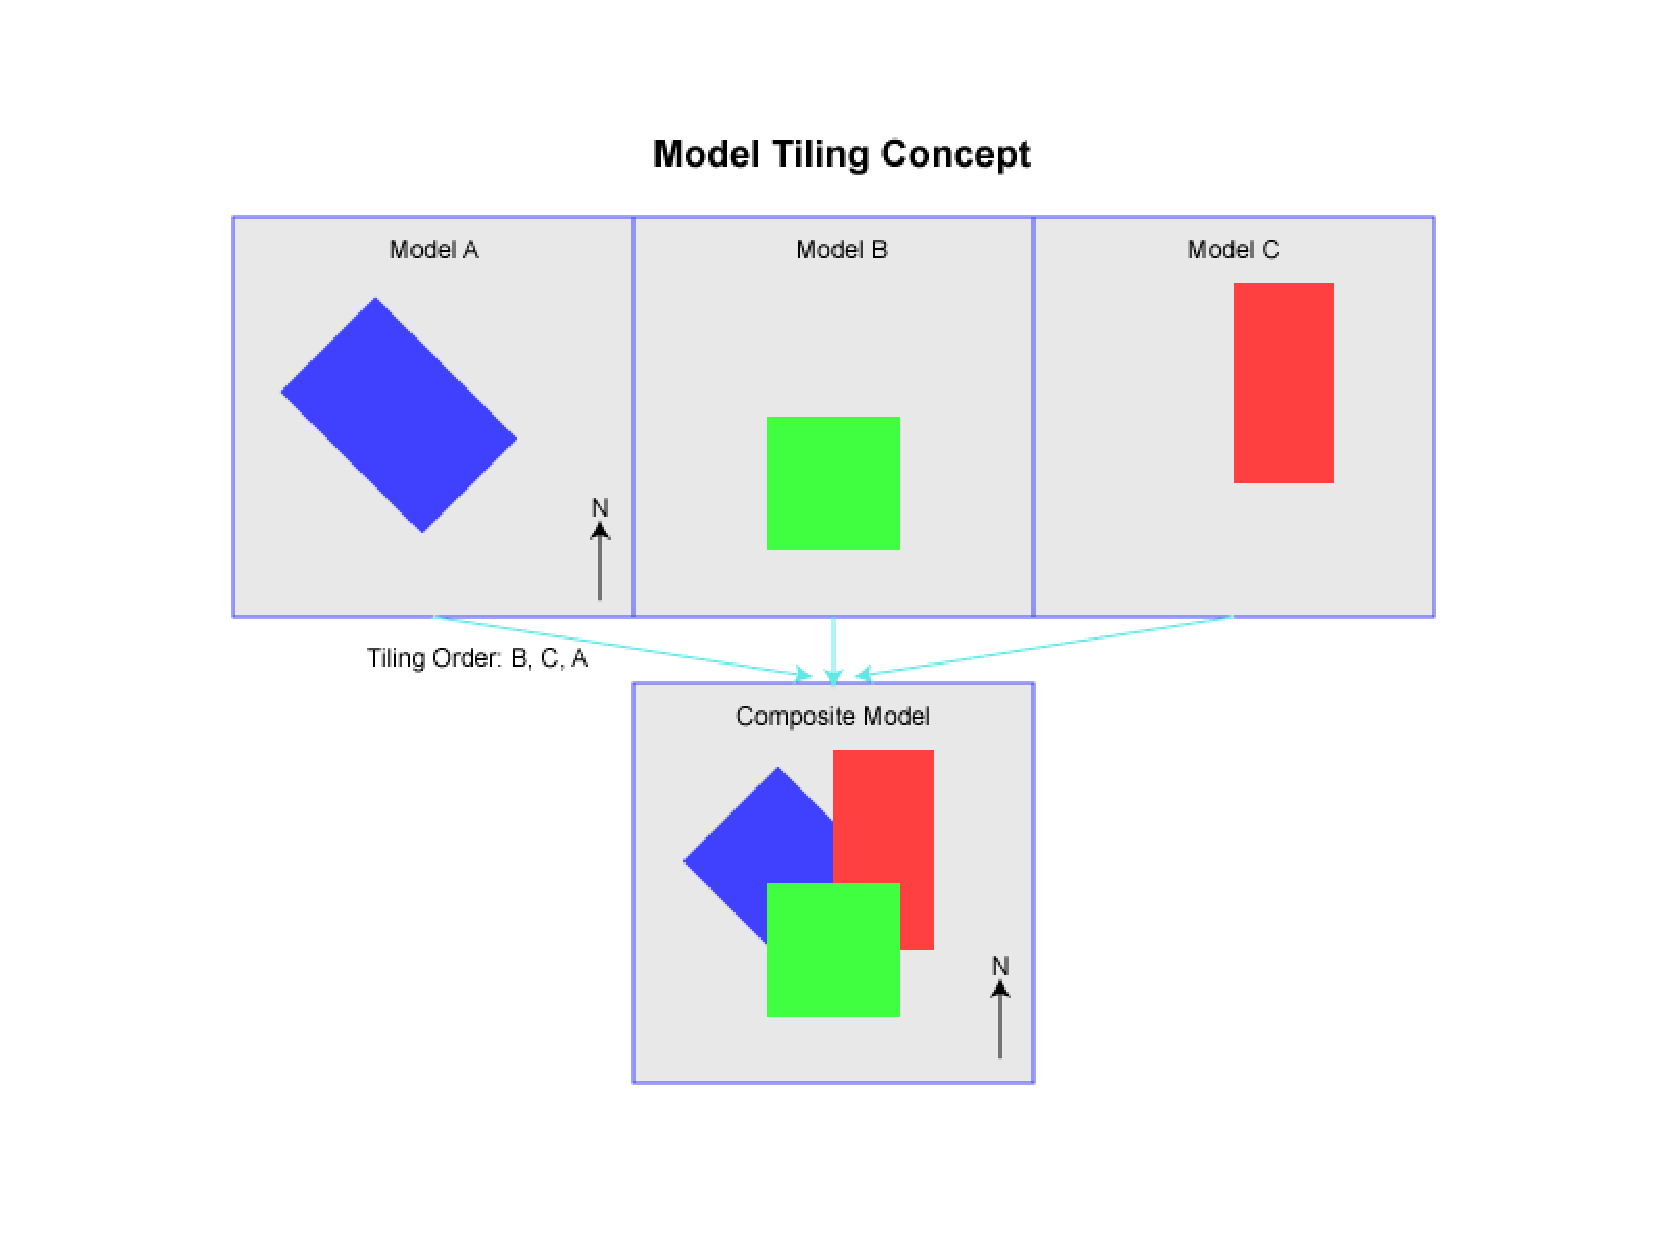
\epsfig{file=UCVM_Tiling_Concept.pdf,scale=0.35}
%\caption{Tiling of velocity models (TODO: Redo/cleanup this figure).}\label{fig:tiling}
%\end{figure}

%The framework further extends the standardized interface by allowing multiple velocity models to be aggregated into a single composite model. Composition is accomplished by tiling two or more velocity models in three dimensions according to a user-specified priority ordering. 
Under this scheme, a query point is submitted sequentially to each velocity model within the ordered list that comprises the composite. The first model to return valid velocity data for the point is considered to have fulfilled the data request and subsequent models are not queried. Thus, overlap among the individual models is acceptable and their relative priority ordering arbitrates which one satisfies any given query. Generally, no smoothing is performed at the interfaces between models (an exception is interpolation between a geotechnical layer and a crustal model as discussed later in this paper). This tiling concept is illustrated in Figure \ref{fig:tiling}.

Community velocity models vary widely in their area of coverage, depth extent, and resolution. UCVM is flexible in its support for such variability. However, in order to better accommodate high frequency ground motion simulations, it categorizes models into two general groups: crustal models, and geotechnical layers (GTLs). Crustal models provide subsurface seismic wave velocities associated with basin, crust, and mantle structures. These models may potentially extend to many tens of kilometers below the Earth's surface yet do so at coarse resolutions (TODO: cite CVM-H, CVM-S). Geotechical layers, in contrast, provide velocities for only the near-surface (typically a few hundred meters) at very high resolution (TODO: cite Ely Vs30 GTL). Ground motion simulations, in particular, rely on high-resolution near-surface velocities and therefore a GTL serves to supplement the coarser data provided by crustal models.

TODO: Interpolation of GTL with Crustal